\documentclass{article}
\usepackage{amsmath, amssymb}
\usepackage[backend=biber]{biblatex}
\usepackage{listings}
\usepackage{color}
\usepackage{xcolor}
\usepackage{graphicx}
\usepackage{tikz}
\usepackage{hyperref}
\usetikzlibrary{trees}

% Define colors for listings
\definecolor{codegreen}{rgb}{0,0.6,0}
\definecolor{codegray}{rgb}{0.5,0.5,0.5}
\definecolor{codepurple}{rgb}{0.58,0,0.82}
\definecolor{backcolour}{rgb}{0.95,0.95,0.92}

% Code listing style
\lstdefinestyle{mystyle}{
    backgroundcolor=\color{backcolour},   
    commentstyle=\color{codegreen},
    keywordstyle=\color{magenta},
    numberstyle=\tiny\color{codegray},
    stringstyle=\color{codepurple},
    basicstyle=\footnotesize,
    breakatwhitespace=false,         
    breaklines=true,                 
    captionpos=b,                    
    keepspaces=true,                 
    numbers=left,                    
    numbersep=5pt,                  
    showspaces=false,                
    showstringspaces=false,
    showtabs=false,                  
    tabsize=2
}

\lstset{style=mystyle}

\addbibresource{references.bib}

\title{Analysis of Binary Search Algorithms}
\author{}
\date{}

\begin{document}

\maketitle

\section{Problem Definition}

The problem is to find the position of a target integer in a sorted array of integers using binary search. If the target is not in the array, the algorithm should return a negative value indicating the target is not present.

\subsection*{Inputs:}
\begin{itemize}
  \item $A$: A sorted array of $n$ integers, where $A[0] \leq A[1] \leq \dots \leq A[n-1]$.
  \item $target$: The integer value we are searching for in the array $A$.
\end{itemize}

\subsection*{Outputs:}
\begin{itemize}
  \item An integer value:
  \begin{itemize}
    \item If $target$ is found in $A$, return the index $i$ such that $A[i] = target$.
    \item If $target$ is not found, return $-1$.
  \end{itemize}
\end{itemize}

\section{Binary Search Algorithms}

\subsection{Non-Recursive Algorithm (Iterative)\cite{chatgpt2023}}
\begin{verbatim}
Algorithm IterativeBinarySearch(A, target)
    Input: An array A, a target integer target
    Output: The index of target in A, or -1 if target is not found

    low = 0
    high = length(A) - 1

    while low <= high do
        mid = low + (high - low) / 2  // Compute the middle index
        if A[mid] == target then
            return mid              // Target found
        else if A[mid] < target then
            low = mid + 1           // Search in the right half
        else
            high = mid - 1          // Search in the left half
    end while

    return -1                        // Target not found
\end{verbatim}

The time complexity of the non-recursive binary search algorithm can be analyzed by considering the operations executed at each step of the algorithm.

\begin{itemize}
    \item \(c_1\): Increment and comparison in the while loop (executed \(n\) times).
    \item \(c_2\): Calculation of mid (executed \(n\) times).
    \item \(c_3\): Comparison of \(A[mid]\) with \(T\) (executed \(n\) times).
    \item \(c_4\): Increment of low (executed \(\sum_{i=2}^{n} t_i\) times, where \(t_i\) is the number of times the target is greater than \(A[mid]\)).
    \item \(c_5\): Decrement of high (executed \(\sum_{i=2}^{n} (t_i - 1)\) times, where \(t_i\) is the number of times the target is less than \(A[mid]\)).
    \item \(c_6\): Return mid (executed \(n - 1\) times in the worst case).
    \item \(c_7\): Return -1 (executed once, only if the target is not found).
\end{itemize}

The running time \(T(n)\) of the algorithm can be expressed as:
\[ T(n) = c_1 n + c_2 n + c_3 n + c_4 \sum_{i=2}^{n} t_i + c_5 \sum_{i=2}^{n} (t_i - 1) + c_6 (n - 1) + c_7 \]

For a given \(n\), \(T(n)\) depends on the values of \(t_i\), which change from instance to instance depending on the input data.

\textbf{Best Case:} When the target is in the middle of the array, the algorithm will terminate in \(O(1)\) time. Here, \(t_i = 1\) for \(i = 2, 3, \ldots, n\), leading to the best-case time function:
\[ T(n) = c_1 + c_2 + c_3 + c_6 + c_7 \]

\textbf{Worst Case:} When the target is not present or located at one of the ends of the array, \(t_i\) can be as large as \(\log n\). Thus, the worst-case time complexity is:
\[ T(n) = c_1 \log n + c_2 \log n + c_3 \log n + c_4 \log n + c_5 (\log n - 1) + c_6 \log n + c_7 \]
This results in a time complexity of \(O(\log n)\).

\subsection{Recursive Algorithm\cite{chatgpt2023}}
The recursive binary search algorithm attempts to find a target value within a sorted array by repeatedly dividing the search interval in half, using a recursive approach. The steps of the algorithm are as follows:

\begin{verbatim}
Algorithm RecursiveBinarySearch(A, low, high, T):
    if high < low:
        return -1
    mid = (low + high) // 2
    if A[mid] < T:
        return RecursiveBinarySearch(A, mid + 1, high, T)
    elif A[mid] > T:
        return RecursiveBinarySearch(A, low, mid - 1, T)
    else:
        return mid
\end{verbatim}

\begin{center}
\begin{tikzpicture}[
  level distance=1.5cm,
  sibling distance=4cm,
  edge from parent/.style={draw,-latex},
  level 1/.style={sibling distance=6cm},
  level 2/.style={sibling distance=3cm},
  level 3/.style={sibling distance=1.5cm},
  level 4/.style={sibling distance=1cm}
  ]

% Root node
\node {\( T(n) \)}
  child {node {\( T\left(\frac{n}{2}\right) \)}
    child {node {\( T\left(\frac{n}{4}\right) \)}
      child {node {\( \vdots \)} 
        child {node {\( T(1) \)}}
      }
    }
    child {node {1}}
  }
  child {node {1}};

\end{tikzpicture}

\[
\begin{aligned}
& \text{At level 0:} \quad T(n) = 1 \cdot T(n) + 0 \cdot 1 \\
& \text{At level 1:} \quad T(n) = 1 \cdot T\left(\frac{n}{2}\right) + 1 \\
& \text{At level 2:} \quad T(n) = 2 \cdot T\left(\frac{n}{4}\right) + 2 \\
& \text{At level 3:} \quad T(n) = 4 \cdot T\left(\frac{n}{8}\right) + 4 \\
& \vdots \\
& \text{At level k:} \quad T(n) = 2^k \cdot T\left(\frac{n}{2^k}\right) + 2^k \\
& \text{Base case:} \quad T(1) = 1
\end{aligned}
\]

The total number of levels in the tree is \( \log_2 n \), and the total time is the sum of the work done at each level:

\[
T(n) = \sum_{k=0}^{\log_2 n} 2^k \cdot 1
\]

The work at each level is constant, \( 1 \), so the total time complexity is:

\[
T(n) = O(\log n)
\]
\end{center}

\subsubsection{Master Method\cite{WinNT}}
We can use the Master Theorem to find the time complexity. Let $T(n)$ be the number of comparisons we perform in the worst case if the input array has $\alpha$ elements. Since we halve the active part and do at most two comparisons in each iteration, the recurrence is:

$$T(n) = T(\frac{n}{2}) + 2$$

The theorem uses the generic form:

$$T(n) = \alpha T(\frac{n}{b}) + f(n)$$

and compares $f(n)$ to $n^{log_b a}$. In our case, $\alpha = 1$ and $\beta = 2$, so $n^{log_b a}$ = $n^{log_b 1}$ = $n^0$ = 1 and $f(n) = 2\exists \mathcal{O}(1)$.

\\

Therefore, it holds that:

$$2 = f(n)\exists \mathcal{O}(1) = \mathcal{O}(n^{log_b 1})$$.

From the Master Theorem, we get the following:

$$T(n) \exists \mathcal{O}(n^{log_b a} log n) = \mathcal{O}(n^0 log n) = \mathcal{O}(log n)$$

\section{Algorithm Implementation}
\subsection{Insertion Sort}
The Insertion Sort algorithm is implemented in Python as follows:
\begin{lstlisting}[language=Python]
    def insertion_sort(
        a:list,
        n:int,
    )->list:
        for i in range(1,n):
            k = a[i]
            j = i - 1
            while j >= 0 and a[j] > k:
                a[j + 1] = a[j]
                ops_insert += 1
                j = j - 1
            a[j + 1] = k
        return a
\end{lstlisting}

For insertion sort, I chose to use a counter indicator inside the while loop as that is the scope of where the taxing operation of moving the values inplace takes place before the insertion.

\subsection{Merge Sort}
The Merge Sort algorithm is implemented with a focus on comparing and merging elements:
\begin{lstlisting}[language=Python]
    def merge(
        a:list, 
        p:int, 
        q:int, 
        r:int,
    )->None:
        nl = q - p + 1  # Number of elements in left subarray
        nr = r - q      # Number of elements in right subarray
        left = [0] * nl
        right = [0] * nr
    
        for i in range(nl):
            left[i] = a[p + i]
        for j in range(nr):
            right[j] = a[q + j + 1]
    
        i = j = 0
        k = p
        while i < nl and j < nr:
            if left[i] <= right[j]:
                a[k] = left[i]
                i += 1
            else:
                a[k] = right[j]
                j += 1
            k += 1
    
        # Copy remaining elements of left, if any
        while i < nl:
            a[k] = left[i]
            i += 1
            k += 1
    
        # Copy remaining elements of right, if any
        while j < nr:
            a[k] = right[j]
            j += 1
            k += 1
    
    def merge_sort(
        a:list, 
        p:int, 
        r:int,
    )->list:
        if p >= r:
            return
        q = (p + r) // 2
        merge_sort(a, p, q)
        merge_sort(a, q + 1, r)
        merge(a, p, q, r)
        return a
\end{lstlisting}

For merge sort, I put a counter operation in the assigning of values to the left and right sub array loops and in the while loop where the core merging of left and right sub arrays takes place. The remaining loops in the merge function is non as consequential to the core merging algorithm as they just assign back to the array whatever is left.

\subsection{Implementation Output}
\begin{center}
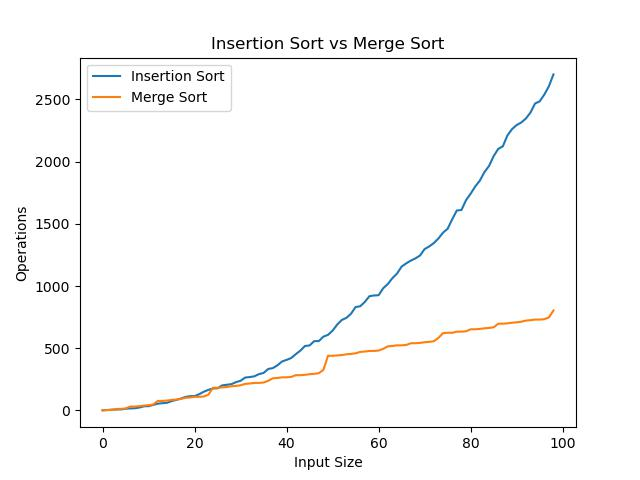
\includegraphics[scale=0.5]{complexity.jpg}
    
\end{center}
This graph depicts the growth of executed operations between insertion sort and merge sort. Insertion sort operation counts are collected every ith loop of n. Merge sort operation counts are collected every 2nd recursive call. 99 operation counters are collected from both insertion sort and merge sort. The actual executed code is found  \href{https://github.com/Tony363/5511/blob/main/hw1/hw1_code.py}{here}
\printbibliography
\end{document}
